\documentclass[10pt]{article}

% Lines beginning with the percent sign are comments
% This file has been commented to help you understand more about LaTeX

% DO NOT EDIT THE LINES BETWEEN THE TWO LONG HORIZONTAL LINES

%---------------------------------------------------------------------------------------------------------

% Packages add extra functionality.
\usepackage{times,graphicx,epstopdf,fancyhdr,amsfonts,amsthm,amsmath,algorithm,algorithmic,xspace,hyperref}
\usepackage[left=1in,top=1in,right=1in,bottom=1in]{geometry}
\usepackage{sect sty}	%For centering section headings
\usepackage{enumerate}	%Allows more labeling options for enumerate environments 
\usepackage{epsfig}
\usepackage[space]{grffile}
\usepackage{booktabs}
\usepackage{forest}
\usepackage{array}
\usepackage{longtable}

% This will set LaTeX to look for figures in the same directory as the .tex file
\graphicspath{.} % The dot means current directory.

\pagestyle{fancy}

\lhead{Final Project}
\rhead{\today}
\lfoot{CSCI 334: Principles of Programming Languages}
\cfoot{\thepage}
\rfoot{Fall 2023}

% Some commands for changing header and footer format
\renewcommand{\headrulewidth}{0.4pt}
\renewcommand{\headwidth}{\textwidth}
\renewcommand{\footrulewidth}{0.4pt}

% These let you use common environments
\newtheorem{claim}{Claim}
\newtheorem{definition}{Definition}
\newtheorem{theorem}{Theorem}
\newtheorem{lemma}{Lemma}
\newtheorem{observation}{Observation}
\newtheorem{question}{Question}

\setlength{\parindent}{0cm}


%---------------------------------------------------------------------------------------------------------

% DON'T CHANGE ANYTHING ABOVE HERE

% Edit below as instructed

\begin{document}
  
\section*{GREG: Great Renderings of Excellent Graphs}

Danny Klein, Austin Osborn

\subsection{Introduction}
    \quad As physics and math students, we have a lot of experience using graphing tools like Mathematica and Desmos. We want to create a language that can graph functions using intuitive input and customizable output. Our language will be able to graph complicated equations in whatever color or style the user desires. Often these complicated equations, like $2x^{(sin(x^2))}$ are incredibly difficult and tedious to graph without the help of a computer, and our language will be able to turn these into easy to read graphs.
    \\ \quad This should have it’s own programming language because it would be incredibly tedious to create these graphs directly in a language not designed for visual output, like F \#, or for graphing complicated equations, like SVG. Examples like Desmos and Mathematica show just how useful this language could be. Our language would make it very easy for users to graph functions, with simple and intuitive programs.

\subsection{Design Principles}
    \quad The primary goal of this language is to provide a method of graphing that is intuitive to use, but still maintains the most important use cases for graphing. When discussing our goals for this project, we brought up several graphing programs that we have used in the past, and features which we appreciated about them as well as features we wished they had with the intent of figuring out a unique space for our language to fall in the landscape of programs we have used. The two primary ones we compared it to were: Desmos and Mathematica. Both of these are substantial programs with complexity of such a degree that it would be near impossible to approximate their functionality in the time we have left this semester, but drawing inspiration from them helped guide our design principles. We seek to make a language which is more intuitive to use than Mathematica (since Mathematica can basically do whatever the user wants as long as the user is able to wade through the dense syntax), but able to do some things that Desmos cannot (since it seems Desmos is on the other end of the spectrum with characteristics fully geared towards intuitiveness, which leaves some customization possibilities at the wayside). 

\subsection{Examples}
\begin{enumerate}
    \item \begin{verbatim}
        Plot (3 + Sin(x)), Solid, Blue. x from -8 to 8.
        We will make a txt file with the command above. Lets call it ex1.txt.
        "dotnet run ex1.txt |> ex1.svg" produces an svg file with the image
        below as output
    \end{verbatim}
    \begin{center}
        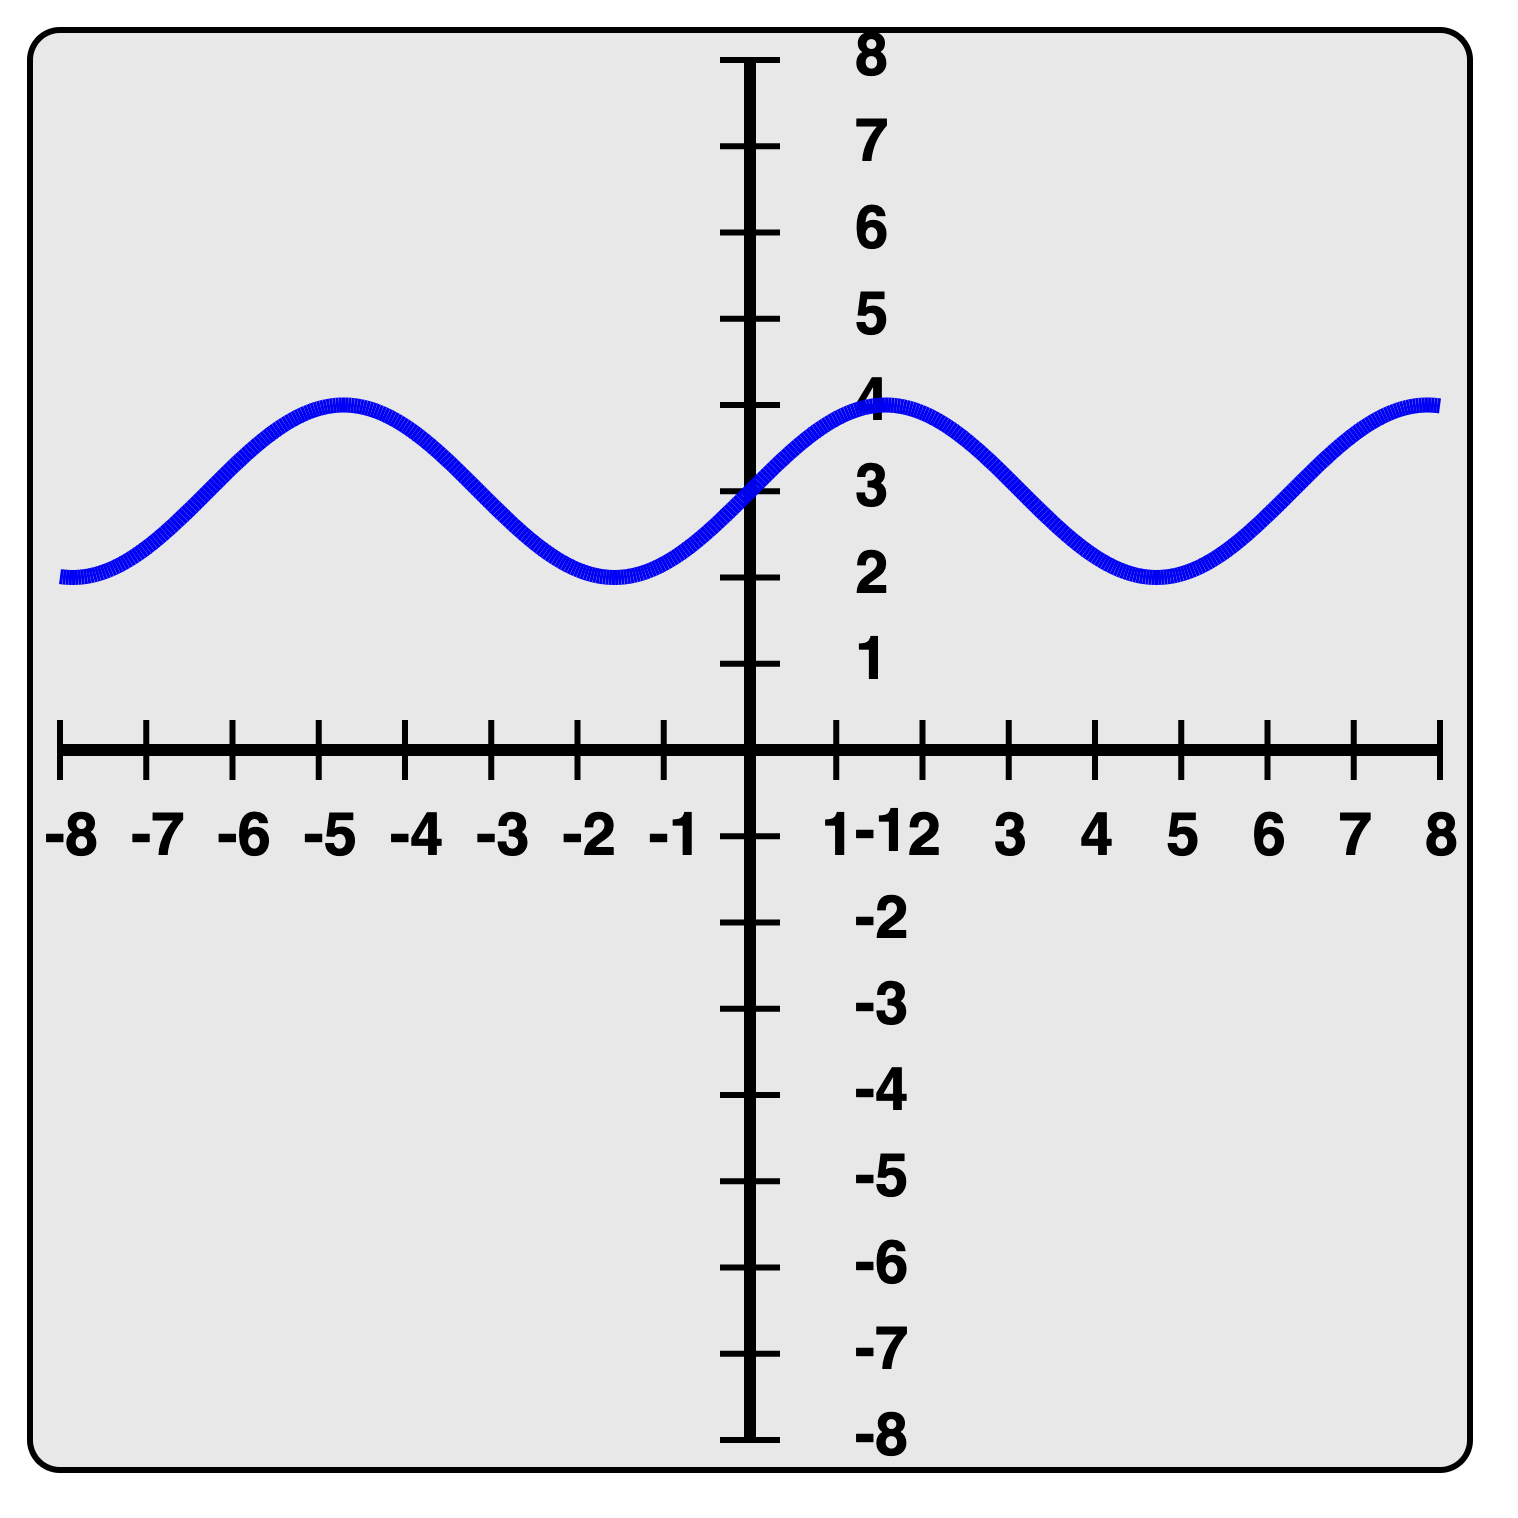
\includegraphics[width = 0.8\textwidth]{ex1.png}
    \end{center}
    \item \begin{verbatim}
        Plot (2/x), Dotted, Green. Plot (x^2)+1, Solid, Blue. Plot (3^sin(x)), 
        Dashed, Red. x from 0 to 5.
        We would put this command in a new txt file called ex2.txt.
        The command "dotnet run ex2.txt |> ex2.svg" produces an svg file 
        that looks like three functions all plotted on the same set of axes.
        We have not yet coded the functionality for dashed and dotted lines, 
        but will add a picture of the output once we do.
    \end{verbatim}
    \item \begin{verbatim}
        Plot 1, Dashed, Black. x from 0 to 1.
        We would put this command in a new txt file called ex3.txt.
        The command "dotnet run ex3.txt |> ex3.svg" produces an svg file 
        of this function, a dotted horizontal line.
        We have not yet coded the functionality for dashed lines, 
        but will add a picture of the output once we do.
    \end{verbatim}
\end{enumerate}

\subsection{Language Concepts}
    \quad The user would not need to understand much to write programs in our language. The user would need to be able to write equations (combining forms) in terms of numbers and variables (primitives), and represent their desired output with a linetype (primitive) and a color (primitive). A user who knows how to write equations, understands colors, and can tell the difference between a solid line and a dashed line, would be able to use our language easily. Our language takes primitives, the numbers and variables, and uses other combining forms such as exponents and trig functions to represent complex equations (combining form), and creates a graphical output (combining form) using the equations along with the color and linetype.
    \\ \quad The only leap necessary from knowing what can be done, to doing it is knowing the specifics of the syntax. This includes: each function beginning with the word Plot, then the function itself, followed by its modifications (linetype and color) separated by commas, followed by a period. Then, we include a domain after all of the functions structured as: variable then range then period. 


\subsection{Syntax}
    \begin{center} 
        \begin{verbatim}
        <Graph>    ::= <Plot>^+ <Domain>.
        <Plot>     ::= Plot <Func>, <Linetype>, <Color>.

        <Func>     ::= <Val> 
                     | <Trig> 
                     | <Op>
                     | <Parens>

        <Val>      ::= <Num>
                     | <Var> 
        <Num>      ::= <Digit>^+ | -<Digit>^+
        <Digit>    ::= 0 | ... | 9
        <Var>      ::= a | ... | z

        <Trig>     ::= <Sin> | <Cos> | <Tan> 
        <Sin>      ::= Sin <Func>
        <Cos>      ::= Cos <Func>
        <Tan>      ::= Tan <Func>

        <Op>       ::= <Plus>
                     | <Minus>
                     | <Times>
                     | <Div>
                     | <Exp>
        <Plus> = (<Func> + <Func>)
        <Minus> = (<Func> - <Func>)
        <Times> = (<Func> * <Func>)
        <Div> = (<Func> / <Func>)
        <Exp> = (<Func> ^ <Func>)
        <Parens> = (<Func>)

        <Linetype> ::= Dashed | Dotted | Solid 
        <Color>    ::= Blue | Green | Red 
                     | Yellow | Purple | Orange 
                     | Black | Gray | Pink
                     | RGB(<Num>, <Num>, <Num>)

        <Domian>   ::= <Var> from <Bound>.
        <Bound>    ::= <Num> to <Num>
        
        \end{verbatim}
        %\includegraphics[width=0.98\textwidth]{images/bnf.jpg}
    \end{center}


\subsection{Semantics}

\begin{center}
    \begin{longtable} { |m{2cm}|m{4cm}|m{1cm}|m{2cm}|m{5cm}| }
        \hline
        Sytnax & Abstract Syntax & Type & Prec./ Assoc. & Meaning \\
        \hline
        x & Var of Char & Char & N/A & x is a primitive, and will represent our independent variable \\
        \hline
        n & Num of int & int & N/A & n is a primitive. We represent integers using the 32-bit integer data type (Int32). \\
        \hline
        Red & Color of Red & String & N/A & Red is a primitive that will represent the color of our line. This is the same for all other Color types besides RGB \\
        \hline
        RGB(200, 200, 200) & Color of RGB & Num* Num* Num & N/A & RGB is a combining form of a 3-tuple of 3 Nums that will represent an RGB color value if someone wants to specify a new color \\
        \hline
        Solid & Color of Solid & String & N/A & Solid is a primitive that will represent the linotype of our line, in this case a solid line. This has the same syntax for the other LineType types, Dashed and Dotted. \\
        \hline
        Val & Num of int or Var of Char & int or char & N/A & Val is a value which can either be a variable or a number. It is used in functions in order to allow for the flexibility requisite for algebraic expressions. \\
        \hline
        Sin x & Trig of Sin & Func & N/A & Sin is a type of Trig, which is a type of Func. It will perform the sine function on x, whatever the inner func is. This has the same syntax for other Trig types \\
        \hline
        (n + m) & Op of Plus & Func * Func & N/A & n + m is a combining form of two funcs, n and m, both of which can be any Func. It will be evaluated as the sum of the two funcs. This has the same syntax for other Op types. \\
        \hline
        Sin(x+(x*2)) & Func of Trig & Func & N/A & Func represents the function that we want to graph. It can be just a val, or more often it is a combining form of many smaller funcs, in this case it includes Sin, Plus, and Exp in addition to the vals x and 2. An infinite amount of unique functions of any length and complexity can be written in this syntax as long as they break down into parts that have been defined above. \\
        \hline
        Plot x, Dashed, Blue. & Plot of \{f: Func; line: LineType; color: Color\} & Record of Func* LineType* Color & N/A & Plot x, Dashed, Blue. is a declaration of a plot which takes the function y = x which will be drawn on a graph with some domain with a blue, dashed line. This syntax is the same for other line types (solid, dotted) and colors (red, yellow…). \\
        \hline
        n to m & Bound of \{lower: Num; upper: Num\} & record of int*int & N/A & n to m is a combining form of two Nums (ints) that represent the lower and upper bound of our domain. It is saved as a record with the first int as lower and the second int as upper. \\
        \hline
        x from n to m & Domain of \{var: Var; bounds: Bound\} & record of char* Bound & N/A & x from n to m is a combining form of a Var (char) and two Nums (ints) that represent the variable, lower bound, and upper bound of our domain. It is saved as a record with the Var as var and the two ints as a Bound record. \\
        \hline
        Plot (2*x), Solid, Red. Plot (3+x), Dashed, Blue. x from -n to n. & Graph of \{plots: Plot list; domain: Domain\} & record of Plot List * Domain & N/A & A Graph is our final combining form, combining our list of Plots with a domain, which will be our input. It is saved as a record of Plot List and Domain. The syntax is the same for any number of plots of different types and any one domain at the end. \\
        \hline
    \end{longtable}
\end{center}

\subsection{Remainig Work}
    \quad We currently have a parser which can parse in a function/domain and make an AST with it, as well as an evaluator which can generate a svg graph of a given domain and draw a function over it if provided with the function. The next step is to combine these two further so the evaluator does not have to be explicitly given a function, but it can be parsed in. Once this is working, all the baseline functionality will be there, and we will be able to focus on implementing extra functionality like color/line type which we have in our docs already, but if those go quickly, more could be added too. 


% DO NOT DELETE ANYTHING BELOW THIS LINE
\end{document}
